\begin{filecontents}{bibtexlogo.sty}

\usepackage[utf8]{inputenc}
\usepackage{graphicx}
\usepackage{amsmath}
\usepackage{svg}
\graphicspath{ {./images/} }
\usepackage{helvet}
\usepackage{subcaption}
\def\lowBibTeX{{\reset@font\rmfamily B\kern-.05em%
    \raise.0ex\hbox{\scshape i\kern-.025em b}\kern-.08em%
    T\kern-.1667em\lower.7ex\hbox{E}\kern-.125emX}}
\def\BibTeX{\protect\lowBibTeX}
\end{filecontents}
%\documentclass[a4paper]{article}
\documentclass[11pt]{article}
\usepackage{harvard}
\usepackage{bibtexlogo}
	\addtolength{\oddsidemargin}{-.500in}
	\addtolength{\evensidemargin}{-.500in}
	\addtolength{\textwidth}{1in}
	\addtolength{\topmargin}{-.500in}
	\addtolength{\textheight}{1in}
\usepackage{helvet}
\newcommand{\comname}[1]{{\bf $\backslash$#1}}
\newcommand{\keyword}[1]{{\bf #1}}
\newcommand{\varname}[1]{{\em #1}}
\newcommand{\harvard}{{\sf harvard}}
\newcommand{\Harvard}{{\sf Harvard}}
\renewcommand{\familydefault}{\sfdefault}
\setlength{\parindent}{0em}
\setlength{\parskip}{1em}

\begin{document}

\begin{titlepage}
   \begin{center}
       %%%%%%%%%%%%%%%%%%%%%%%%%%%%%%%%%%%%%%%%%%%%%%%%%%%%%%%
       \large
        
\includegraphics[scale=0.4]{logo}
       \\
       \vspace{0.5cm}
        SCHOOL OF ENGINEERING \\
        \vspace{0.5cm}
        YEAR 3 INDIVIDUAL PROJECT
        
        
            
       \vspace{1.5cm}

       \underline{\textbf{INTERIM REPORT}}\\
       \vspace{1.5cm}
       \Large{3D-printed Origami Solar Sails for Next Generation of CubeSats: Multi-body folding dynamics}
       \normalsize
       
      
       \vspace{1cm}
       Project no. 201
       \\
       

       \vfill
        
        \large
       Raymond Arturo Minarro Escalona
            \\
        BEng Aerospace Engineering with Year in Industry (H426)
        \\
        Monday 8th of February, 2021
       \vspace{0.8cm}
    
       \large{Supervisor: Soldini, S.}
       \normalsize
       %%%%%%%%%%%%%%%%%%%%%%%%%%%%%%%%%%%%%%%%%%%%%%%%%%%%%%%
   \end{center}
\end{titlepage}

\bibliographystyle{agsm}

%\tableofcontents
\pagebreak
%%%%%%%%%%%%%%%%%%%%%%%%%%%%%%%%%%%%



%%%%%%%%%%%%%%%%%%%%%%%%%%%%%%%%%%%%%%%%%%%%%%%%%%%%%%%


\section{Experimental project approach and methods }

The purpose of the project
is to deploy a set of connected, 3D printed panels that convert into a sail large enough to impulse the vessel in a direction normal to
sun. In this report, a Python software has been under development to study the speed, dampening and restive behaviour of the panels when extended by the solar radiation pressure. This will later on evolve onto a more complex simulation with the aim of studying the folding dynamics of a 3D printable sail. A set of aims are:

\begin{itemize}
    \item To study the multi-body dynamic behaviour of the deploying panels;
    \item To study the feasibility of more arrangements of unfolding panels to be used in the final design;
    \item To understand the physical principles governing the attitude control and impulse of the cubesat in deep space missions;
    \item To study the efficacy of using SRP as source of impulse in deep space without the need for fuel.
\end{itemize}

\subsection{Physics}

In this problem, common rotational physical principles are used to rotate reference frames assigned to the different panels and the bus of the cubesat, the dynamic system after which the simulation is modelled is iterated and described in each type of simulation below.

The bus is defined as a prism by common expected dimensions of 0.43m by 0.93m by 0.43m (width, length and depth respectively.) and a panel dimensions of length $l=0.7m$ and height of $h=0.7m$. These are preliminary specifications and will be changed once an optimal structure is found.

The panel is assumed to be similar to high-end domestic polyactic acid (PLA) 3D printed layers of $50\mu m$. 3D PLA printers work by heating up PLA filament and setting it on a work surface close to each other to cool and form a solid, layered shape. For a PLA filament of $\rho_{PLA} = 1.24g/cm^3$ \protect\cite{pladensity} then the panel will have an area-density according to eq. \ref{density}

\begin{equation}
\rho_{A_{PLA}} = \rho_{PLA} t = 1240 kg/m^3 \cdot 50 \cdot 10^{-6} m = 0.062 kg/m^2 \label{density}
\end{equation}

With a moment of inertia, for a rectangle about one of its edges:
\begin{equation}
    I_{zz}= \frac{1}{3} m*l = \frac{1}{3} l^2h\rho_{A_{PLA}} = 7.09\cdot10^{-7} 
\label{inertia}
\end{equation}

\subsection{Solar Radiation Pressure} \label{srp}

The pressure on a theoretical flat zone, normal to the sun, reaches a value of:

\begin{equation}
p = G_{sc}/c = 5.97 \mu N/m^2
\label{Gsc}
\end{equation}
Where $G_{sc}$ is the solar constant, and $c$ is the speed of light \protect\cite{solarhandbook}. 

The solar constant is used in astrophysics to identify the
energy carried by photos expelled from the sun, measured as
flux density at an average Earth-Sun distance nominated as an
astronomical unit (AU), 1 AU has a fixed value of $1.49\cdot10^{11}$ meters \protect\cite{Astro}

Given that the energy is propagated radially as a sphere away from the sun, the energy decrease is inversely proportional to the distance. As such, the inverse square law is applied to eq. \ref{Gsc} to find the equivalent pressure at a distance of $R_s$ (eq. \ref{angledp}), multiplied by the cosine of the angle $\alpha$ between the sun frame and the bus frame \protect\cite{sundyn}

\begin{equation}
p_{bus} = \frac{p}{R_s^2} cos(\alpha) = \frac{G_{sc}}{c R_s^2} cos(\alpha)
\label{angledp}
\end{equation}

Afterwards, this equivalent pressure $p_{bus}$ may be translated into a force acting on each panel ("panel" frame of reference) which may be oriented initially at an angle $\beta$ away from the bus frame, in addition to a state-trigger variable $d$ to model the RCDs \protect\cite{attitudeAndres}, giving eq. \ref{totalFsrp}
\begin{equation}
F_{srp} = cos(\beta)p_{bus}A_{panel}(1+d) = \frac{G_{sc}}{c R_s} cos(\alpha)cos(\beta)A_{panel}(1+d)
\label{totalFsrp}
\end{equation}

At this point, from the force normal to the panel, further mechanical simulation values may be derived.

\subsection{Simulation}

At the current stage of development, a simulation script has been under development in Python utilising libraries like SymPy allows the use virtual reference frames for the sun, bus and panel components, these panels may be rotated and translated during the simulation calculation (Figure \ref{fig:sim_frames})

\begin{figure}[!htb]
\centering
\begin{subfigure}{0.5\textwidth}
  \centering
  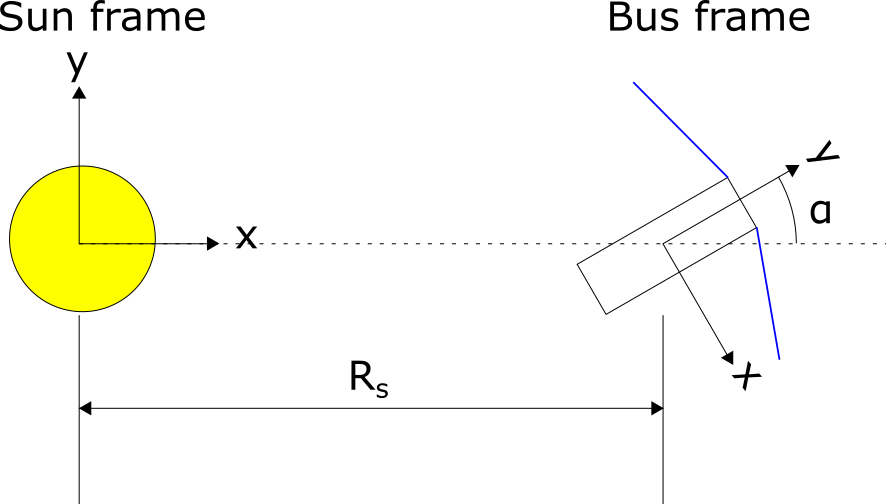
\includegraphics[width=0.7\linewidth]{images/sun bus frames.png}
\end{subfigure}%
\begin{subfigure}{.5\textwidth}
  \centering
  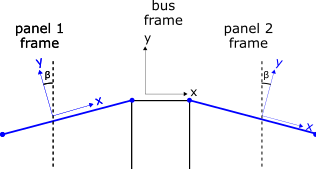
\includegraphics[width=0.7\linewidth]{images/bus panel frames.png}
\end{subfigure}
\caption{Reference frames within the simulation. Blue elements are panels (fully reflecting, $d = 1$) and black elements represent the bus of the CubeSat.}
\label{fig:sim_frames}
\end{figure}

In the discipline of physics and mechanic simulations there exists different methodology and basis by which different types of simulations arrive to a solution, or lack thereof.


Different methods use different amount of resources and have different solving times depending on the complexity of the problem \protect\cite{simulations}. For the routine herein, a time-discrete state-space continuous is used.

\begin{itemize}
    \item \textbf{Time discrete}: The simulation begins at an initial state, which may be configured using the variables defined in \ref{srp}. The variables are refreshed every time-step and handled accordingly. The process is repeated until a desired variable "converges", e.g the number of sig\-ni\-fi\-cant figures desired do not change anymore between time-steps, and any further step taken only increases the precision (not necessarily accuracy).
    \item \textbf{State-space continuous}: The variables calculated therein fall within the spectrum of values the simulation range is working with, giving calculations the liberty of yielding more precise values.
\end{itemize}

As outlined above, the simulations were carried out in discrete time jumps, and a continuous state-space system. Variables like $F_{srp}$ panel torque $T_{p_n}$, angular acceleration $\alpha_{p_n}$, angular speed $\omega_{p_n}$ where calculated each cycle or time-step of $3.6s$. The time-step was chosen as a compromise between solve time and simulation of the system with real-life values, which are slow-acting due to the nature of the solar radiation pressure.
Given the problem summary, the forces acting on a panel assimilate to how forces on a pin-ended beam would behave, adding a torsional spring $-k\theta$ that opposes the torque $T_{p_n}$ caused by the force $F_{srp}$. An analogue system using a mass $m$ being pushed by $F_{srp}$ against a spring $kx$ causing a displacement $x$ was used and modelled.

The equivalent newtonian governing equation for the translational system is:

\begin{equation}
    m\ddot{x} = F_{SRP} - kx
\end{equation}


and its rotational Euler equation:
\begin{equation}
I_{zz} \ddot{\theta} = T_{SRP} - k\theta
\end{equation}


\section{Results to date}
\subsubsection{Initial simulation system}


After the simulation terminated due to the value of $\theta$ reaching 90 degrees as seen in figure \ref{fig:1_results}, at which point it would start clipping the bus or folding "backwards", it was seen that the panel was oscillating and never converged. 

\begin{figure}[!htb]
\centering
\begin{subfigure}{0.5\textwidth}
  \centering
  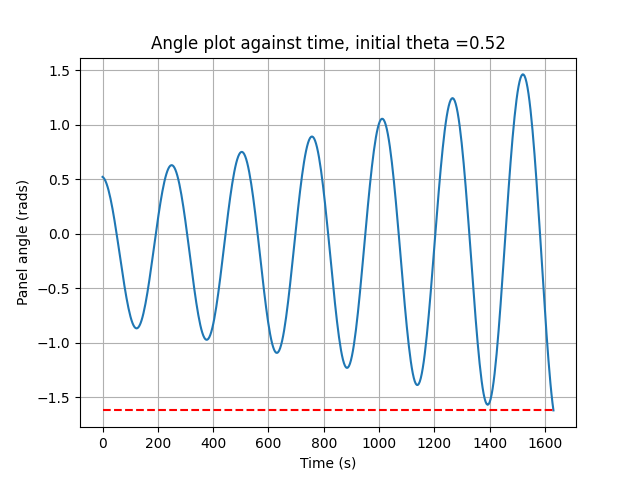
\includegraphics[width=1\linewidth]{images/first/theta_plot.png}
  \label{fig:1_theta}
\end{subfigure}%
\begin{subfigure}{.5\textwidth}
  \centering
  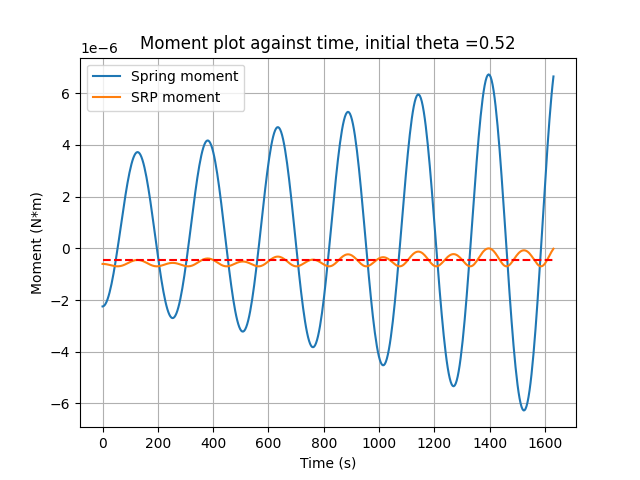
\includegraphics[width=1\linewidth]{images/first/moment_plot.png}
  \label{fig:1_moment}
\end{subfigure}
\caption{Simulation 1, the panel starts at a $\theta = 0.52 rads$ and does not converge.}
\label{fig:1_results}
\end{figure}



After further research, the initial system by which the simulation was mo\-del\-led represented a second-order dynamic system with a governing equation similar to a second-order ordinary differential equation:

\begin{equation}
f''(x) + af'(x) + bf(x) = u \label{dyneq}
\end{equation}
Where:
$$a = 2 \zeta \omega_n ; b = \omega_n^2$$

However, as there is not a $af'(x)$ factor, upon which depends the damping ratio $\zeta$, the present system would oscillate at a frequency of $\sqrt{k/I_{zz}}$

These results indicate that, in real life, the system would have to have a mechanism to stop it from oscillating, be it a damper, or a system that counter-acts moment proportional to angular speed $\omega$ or $\dot{\theta}$. The reason why the amplitude of the oscillation increases is related to the limited minimum amount the system can accelerate every time-step, a smaller time-step would yield a system oscillating at a fixed amplitude.

Alternatively, such solution may be achieved by a electrically-controlled spring, which may activate/deactivate at its full spring coefficient $k$ frequently enough to maintain a neutral angular speed and therefore facing angle.

\subsubsection{Controllable spring simulation}



Instead of the spring being active permanently, an exception to the simulation may be added in such way that:

\begin{figure}[!htb]
\centering
\begin{subfigure}{0.5\textwidth}
  \centering
  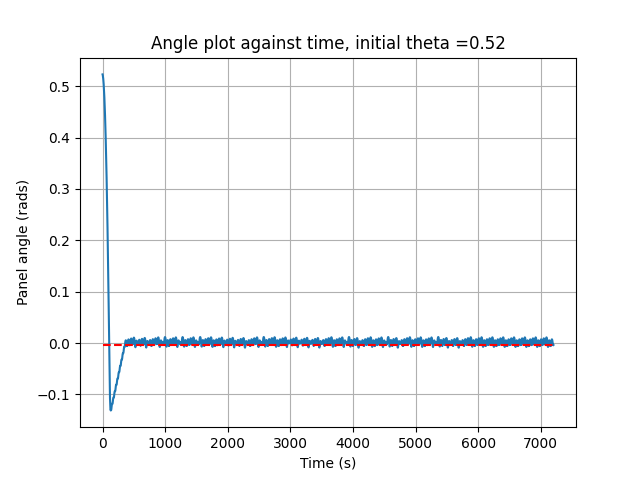
\includegraphics[width=1\linewidth]{images/second/theta_plot.png}
\end{subfigure}%
\begin{subfigure}{.5\textwidth}
  \centering
  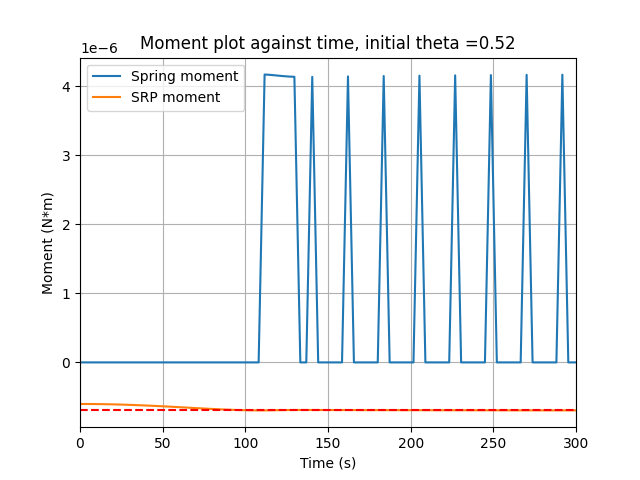
\includegraphics[width=1\linewidth]{images/second/moment_plot.png}
\end{subfigure}
\caption{Simulation 2 where in the spring is electrically activated. Resulted in a small converged value around which $\theta$ oscillates.}
\label{fig:2_results}
\end{figure}

$$ \alpha < 0 \implies k = k_{s}$$
$$ \alpha \geq 0 \implies k = 0$$

This means that, when $\alpha$ is negative (accelerating forward towards the sail facing direction), the spring activates and delivers a moment (eq. \ref{moment spring}), as it can be seen in figure \ref{fig:2_results}

\begin{equation}
    M_{spring} = -k\theta \label{moment spring}
\end{equation}

\begin{figure}[!htb]
\centering
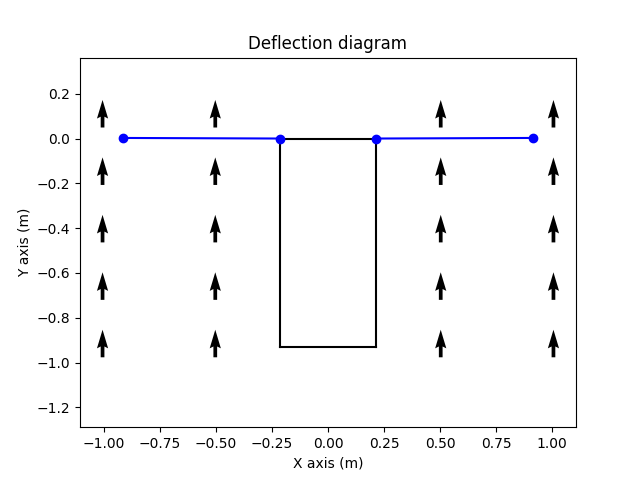
\includegraphics[width=0.5\textwidth]{images/second/deflection_diagram.png}
\caption{"Approximate" converged diagram for Simulation 2. The panels oscillate close to a value of $\theta = 0$ where $F_{srp}$ is the greatest.}
\label{fig:2_diagram}
\end{figure}

It is worth noting that due to $M_{spring}$ being far larger in magnitude than $T_{p_n}$, a single time-step is enough to cause a $\delta\alpha$ larger than the negative value of $\alpha$ that triggered the spring, driving the panel at a uniform pace until an angle of $\theta = 0$ is reached (See final "approximate" state in figure \ref{fig:2_diagram}. This will yield a spring moment of 0 when triggered, self-balancing the system in a constant, small oscillation proportional to the time-step of the simulation.

This resulted on a system that oscillates around the converged value for $\theta$, as with the first simulation, the amplitude of the post-convergence oscillation is proportional to the minimum amount of acceleration in one time-step.

\subsubsection{Passively damped simulation}

Following the suggestions of adding a dampening mechanism to comply with the dynamic equation \ref{dyneq} describing a second-order system, an arbitrary value of $\zeta = 0.45$ is chosen for the new system (Figure \ref{fig:3_system}), and the simulation tweaked to take this into consideration.

%The new dynamical system equivalent (Figure \ref{fig:dampspring} %has a damper with coefficient adjusted to achieve the $\zeta$ %value desired.

%\begin{figure}[h]
%\centering
%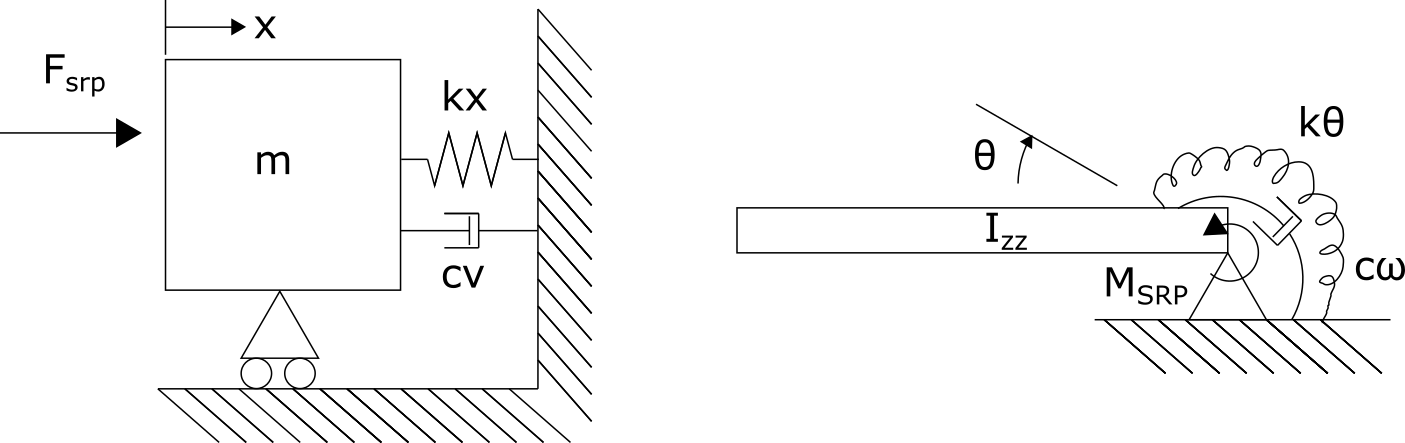
\includegraphics[width=\textwidth]{images/spring damp system.png}
%\caption{New equivalent dampened dynamic configuration} %\label{fig:dampspring}
%\end{figure}
%

\begin{figure}[!htb]
\centering
\begin{subfigure}{0.5\textwidth}
  \centering
  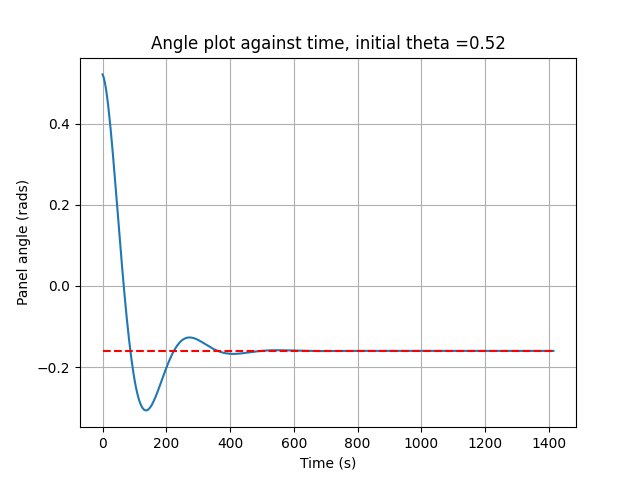
\includegraphics[width=1\linewidth]{images/third/theta_plot.png}
  \label{fig:3_theta}
\end{subfigure}%
\begin{subfigure}{.5\textwidth}
  \centering
  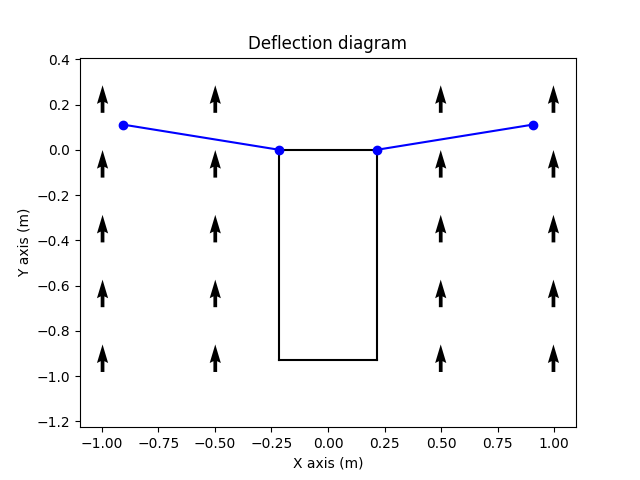
\includegraphics[width=1\linewidth]{images/third/deflection_diagram.png}
  \label{fig:3_deflection}
\end{subfigure}
\caption{Simulation 3 with passive dampening of $c\omega$, the angle converged faster and definitely where the sum of moments balances out.}
\label{fig:3_results}
\end{figure}

As shown in figure \ref{fig:3_results}, the angle converged faster thanks to the dampening in the system, yielding a precise offset angle where the moment of the spring is balanced out by the torque of the panel, this offset decreases slightly the total force achievable, as noted by the higher moment peak. The final state converges at a point where $M_{spring} = T_{p_n}$, yielding a lower value of $F_{srp}$ than simulation 2.

\begin{figure}[!htb]
\centering
\begin{subfigure}{0.5\textwidth}
  \centering
  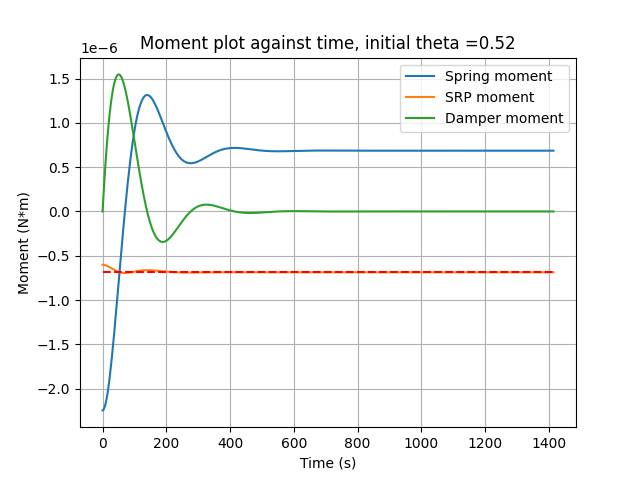
\includegraphics[width=0.7\linewidth]{images/third/moment_plot.png}
  \label{fig:3_moment}
\end{subfigure}%
\begin{subfigure}{.5\textwidth}
  \centering
  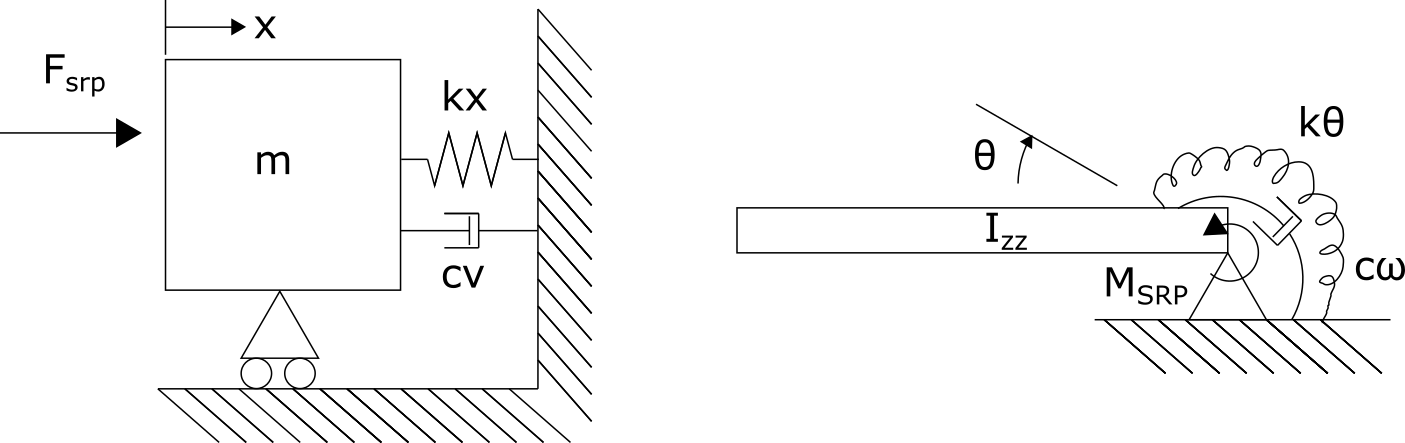
\includegraphics[width=1\linewidth]{images/spring damp system.png}
  \label{fig:3_dynsym}
\end{subfigure}
\caption{Simulation 3 new dynamic-equivalent system and moment plot obtained, note the spring moment being equally opposite to the SRP moment when the damper moment settles. }
\label{fig:3_system}
\end{figure}

\section{Work programme}

All items to this day are done, kick-off meetings, GIT repo set-up and proposal submission achieved. Making exception for
some items in the December-January have had their deadlines extended. After revision
of the Gantt chart, it was decided that items such as "literature review", "principles studies and testing" "liaison for design" "requirement gathering" and "code development" are continuous and concurrent up until the "new code testing and debugging" date. Items "Available code review" and "Available code testing" were moved towards march as it is ideal that the researcher begins the code by understanding the principles from scratch, and then consulting other sources.


\section{Future plans}

From the results seen from this simulation, it is safe to move forward and extend the code to several connected panels, which may make each cycle have a heavier calculation load, as each cycle and moment calculation will have to consider the motion of the next panel over.

The code, which utilises Reference Frames with three axes, x, y and z, may be adapted to recreate 3D arrangements, for which team liaison must be done to consider the 3D folding possibilities being worked by another member of the project.

Checks need to be made to verify the sizes of the sails needed and the trade with weight are appropriate enough to achieve the orbital transference desired by mission control, which is being worked by another member of the project.

A model can be cloned and simulated into Mathworks' Simscale to validate the Python model and enhance the understanding of the multi-body dynamics.
\pagebreak
\bibliography{harvard}

\appendix
\pagebreak
\section{Revised Gantt Chart}

\end{document}
